\documentclass[12pt]{article}

\usepackage{sectsty}
\usepackage{fullpage}
\usepackage{graphicx}

\sectionfont{\large}
\begin{document}\vspace{0.5in}
\begin{center}\begin{large}\textbf{Jatin Mittal}\end{large}\end{center}\textbf{\hrulefill}\\

\begin{tabular}{@{}p{4in}p{3in}}
Room No-A6 & {Phone:}+91-7753820670 \\
Dr. S RadhaKrishnan Hostel & {E-mail:}jatinmittal199510@gmail.com\\
University of Allahabad \\
Allahabad\\
& 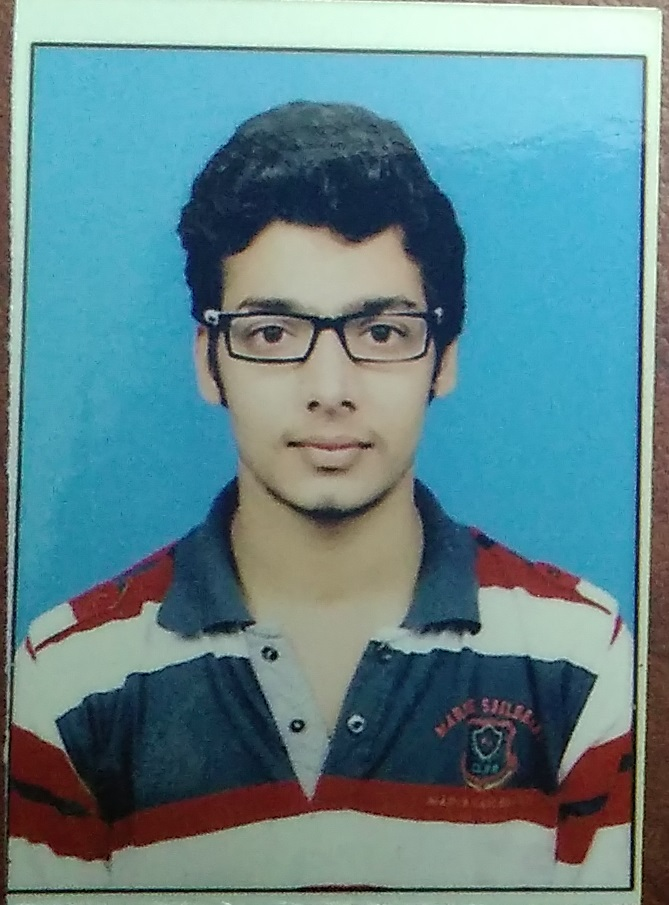
\includegraphics[scale=0.2]{my.jpg}\\
\end{tabular}

\section*{Objective}
To work at an esteemed organization to enhance my knowledge \& skills by achieving professional \& personal growth in all aspects of life \& completing whatever responsibilities undertaken with optimistic view, experience \& best of my efficiency. 
\section*{Education}
\begin{tabular}{|l|l|l|l|l|}
\hline
Degree & College/School & University & Passing Year & Pass Percentage\\
\hline
B. Tech & JKIAPT & Allahabad University & 2017 & 72.12 (till 5th sem)\\
\hline
Intermediate & Silver Line School & CBSE & 2013 & 93.40\\
\hline
High School & St. Mary's Convent School & ICSE & 2011 & 85.14\\
\hline
\end{tabular}

\section*{Projects}
\begin{itemize}
\item[$\bullet$]\textbf{Hotel Guest Service Robot.}\\November 2015- Feb 2016\\Members: Abhishek Rathore, Gorji P. Sampath, Aditya Kumar

This project was based on Atmega 2560 to provide the automatic services to the Hotel Guests as per their need. We won the first position in e-YRC competition amongst many other teams that participated.
\item[$\bullet$]\textbf{'J.K. Results' android App.}\\Oct 2015- Jan 2016\\
This project was the part of my Semester projects. This app was developed considering the need to have the results on students phone.
\item[$\bullet$]\textbf{'Automated' anroid App.}\\May 2015-July 2015\\
This application was developed to make some features of the phone as automatic. For example, turning wifi on, connecting to a specified network, turning it off at the particular time of the day as per the settings made.
\end{itemize}
\section*{Technical Skills}
\begin{itemize}
\item[$\cdot$]Programming Languages
\begin{enumerate}
\item C
\item html,css
\item Java
\end{enumerate}
\item[$\cdot$]Knowledge of Data Structures and Algorithms.
\item[$\cdot$]Tools and Technologies Used
\begin{enumerate}
\item Parse Database
\item Atmel Studio
\item Android Studio
\end{enumerate}
\end{itemize}
\begin{itemize}
\item[$\cdot$]
\end{itemize}
\section*{Soft Skills}
\begin{itemize}
\item[$\cdot$]Good and Persuasive Communication Skills.
\item[$\cdot$]Optimistic person with an ability to work under pressure with a ‘Never Giving Up’ tendency.
\item[$\cdot$]Proficient in grasping new technical concepts \& utilizing them in effective manner.
\end{itemize}
\section*{Extra-Curricular Activities}
\begin{itemize}
\item[$\cdot$]Robotics Competition.
\end{itemize}
\section*{Co-Curricular Activities}
\begin{itemize}
\item[$\cdot$] Playing Chess, Kho-Kho, Badminton
\item[$\cdot$] Listening Music
 \end{itemize}
\section*{Personal Details}
\begin{itemize}
\item[$\cdot$]Father's Name : Mr. S.K. Mittal
\item[$\cdot$]Mother's Name : Mrs. Ruchi Mittal
\item[$\cdot$]Sex           : Male
\item[$\cdot$]Date of Birth : February 26,1995
\item[$\cdot$]Nationality   : Indian
\item[$\cdot$]Martial Status: Single
\end{itemize}
\section*{Declaration} I hereby declare that the above information is true and authentic to the best of my knowledge.
\section*{Date} May 25,2016

\end{document}